\bigpicgeometry
\thispagestyle{empty}
\vspace*{\fill}
\begin{center}
	\label{elder-joseph-bed}
	\includegraphics[width=4.25in]{./Images/Elder_Joseph_Bed.png}

	The Elder Joseph shortly before his repose
\end{center}
\vspace*{\fill}\restoregeometry
\titleformat
	{\part} % command
	[display] % shape
	{\bfseries\Large} % format
	{
		\begin{center}
		\thepart
		\end{center}
	}
	{0.5cm}
	{
		\vspace{-1.5cm}
		\begin{center}
			\color{red}
	} % before-code
	[
			\color{black}
			\vspace{1cm}
			\bfseries\normalsize		
			The poor offering of a spiritual son to the\\memory of an unforgettable Father\\
			\vspace{2cm}
			{\includegraphics[height=5cm]{./Images/Part_Emblem.png}}
		\end{center}
	]
	
\part{The Life\\of the Optina Elder\\HIERO-SCHEMAMONK JOSEPH}

\newpage
\begin{center}
	\includegraphics[width=\the\textwidth]{./Images/Chapter_Banner.png}\\
	\vspace{1.5cm}
\end{center}
\hugered{A}FTER THE REPOSE of Batiushka Fr. Joseph, I began to receive many letters from relatives, acquaintances, and persons completely unknown to me--all with one and the same request: to describe to them in greater detail the final moments and the burial of Batiushka, and to relate what was known to me of his biography. These letters became so many that, having answered two or three letters with haste, I suddenly felt utterly unable to satisfy everyone with my answers--a fresh wound is still too sensitive. The inevitable contact with recent sorrowful events through their recounting in my letters called forth memories too painful for my heart. The thought that was looming within me, to leave unanswered the letters which I had received, was quickly dispelled by pangs of conscience. I thought to substitute for the letters some short publications concerning the life and repose of Batiushka, but unfortunately, other than ``The Sermon at the Grave'' (in its printed form quite different from that in which it was spoken at Batiushka's burial), and a very brief article conveying nothing either to the heart or to the mind--apart from these nothing printed concerning Batiushka had appeared!

Whereupon, having taken a blessing at his dear little grave, I decided to relive once more in my soul the grievous loss, and by means of the printed word to answer the inquiries of all who had turned to me. By this I hoped, first of all, to satisfy their desire, which I understood so well, to know something of the life of the beloved Elder. And, secondly, I wished to honor with my own contribution, however small it might be, the dear memory of him by whose kindness and encouragement in the course of so many years I, the worst of his spiritual children, had profited.

Batiushka was born on November 2, 1837, in the village of Pokrov of the Starobelsk District of the Kharkov Province. His parents, Evfimy and Maria Litovkin, were very pious people who tried to raise their children in the fear of God. There were six children, three daughters and three sons, of whom Batiushka was the middle child.

Evfimy Litovkin was from a well-to-do peasant Cossack family. For a long time he had held the position of village-head and enjoyed the respect of all, Maria was from a family of the clergy. Both very much loved to help the poor, and often did this without the other's knowledge. They especially venerated Saint John the Almsgiver, in whose honor Batiushka had been named.

Batiushka's father secretly desired that some one of his children enter the monastic life, and the Lord fulfilled this desire in the person, firstly, of his daughter Alexandra, and later also in the person of Batiushka. (His daughter Alexandra entered the Borisovsk Women's Hermitage in the Kursk Province. She led an exalted spiritual life, even served as an Eldress, and reposed as a schema-nun with the name Leonida.) Batiushka loved to recall his childhood, and himself would relate how on feast days his mother would wake all the children for Matins, and after returning from church, between Matins and the Liturgy she would make Batiushka read an \textit{akathist} aloud, while she herself censed throughout the house. Batiushka would say, ``Ooh! She was strict! She was more like a man than a woman.''

Concerning his father Batiushka would say that he was, on the contrary, of a lenient character and was reluctant to punish the children. When Mother Leonida, at the beginning of her monastic life, was subjected to great temptations and thought of leaving the convent, her mother, who had just reposed, appeared to her during sleep and sternly reproved her, reminding her of her monastic vows.

When Mother Leonida told Batiushka Fr. Amvrosy about this, he said to her, ``Your mother is a saint!''

Batiushka's father reposed in 1841, and in 1848 his mother reposed from cholera. Batiushka himself related to me that she was the first in their village to die from this epidemic and the first to be buried in the farther cemetery.

Being left an orphan, Batiushka had to undergo and endure much that was grievous, first from his older brother and later from various masters for whom he worked. Moving from one city to another, and traveling the distance between them on foot, Batiushka endured both hunger and cold. How many times in the inclement autumn weather his feet were soaking wet and frostbitten, and he ate nothing for several days at a time.

Once, being exhausted by the long walk and by hunger, Batiushka entered a certain village; at the entrance to the village, two Cossack women were selling bread. One of them caught sight of the exhausted and scrawny young wayfarer; her sensitive heart was filled with pity, and turning to her friend, she said, ``The poor one! He's probably hungry; let's give him some bread!'' and with these words she gave Batiushka a hot soft roll. In relating this incident not so very long ago to one nun, Batiushka said that to the present time he remembers with thanksgiving those kind women and what they did for him. The compassionate Cossack women, to whose lot fell the good fortune of showing such a kindness to the future great Elder, did not even suspect that by this act of almsgiving they had perhaps entrusted themselves for eternity to his holy prayers for their salvation.

Batiushka found himself in Taganrog and in Rostov; he worked in the tavern of an Armenian in Nakhichevan, and finally wound up at the mill of a certain pious old miller who loved to attend the church services and to read spiritual books, and he never hindered Batiushka from doing the same. From childhood Batiushka loved church, and wherever he lived, on feast days he always tried to be at the Liturgy; hence, his life at the mill was much to his liking.

From there he thought to go to Kiev to venerate the saints of God who repose there, but on the way he stopped at the Borisovsk Hermitage to visit his sister. She persuaded him to go first to Optina and provided him with letters to Batiushka Fr. Amvrosy who had just then entered upon the struggle of eldership after the death of his guide, Batiushka Fr. Makary.

Batiushka Fr. Joseph went to Optina in 1861 on the first of March, ``On Evdokia'' (i.e., on Saint Evdokia's day), as Batiushka would often say. In accord with the counsel of the Elder, he remained at Optina where he was straightway received into the brotherhood of the skete and put to work in the skete kitchen where he remained until Trinity Day.\trans{The Sunday of Pentecost.}

On this day, which was to be significant for him, he was appointed as cell-attendant to the Elder Batiushka Fr. Amvrosy and from that time he spent thirty years inseparable from his great teacher and father.

Batiushka's pious attachment to Fr. Amvrosy was most moving. Batiushka always spoke of him with a smile of tender compunction, and when it happened that you would ask his help and holy prayers in some important matter, he would often advise, ``And you ask Batiushka, too!'' In his instructions also he loved to cite the words of his departed Elder.

Concerning Batiushka's life as cell-attendant for the Elder Amvrosy I know little, but I have heard from many that as a cell-attendant he was irreplaceable. Always distinguished by his extraordinary accuracy and precision in fulfilling his duties, Batiushka always related the Elder's answer word for word to those who made inquiries through him, for which cause the nuns who came to the Elder especially loved him, and if it was difficult to get to the Elder, infirm and burdened as he was by the multitudes of people, then they would summon Batiushka and through him receive the most precise answers. Likewise, many turned to Batiushka Fr. Amvrosy by writing letters which were presented to him by Batiushka Fr. Joseph, who faithfully conveyed Batiushka's answers to all the points of each letter.

Batiushka was always distinguished for his reserve and silence in dealing with visitors, and unless he found it absolutely necessary, he would rarely go out to the people in the hut. In 1884, Batiushka was ordained hieromonk, and from that time on Batiushka Fr. Amvrosy began to send the nuns to him for confession.

When Batiushka was still a hierodeacon, Fr. Amvrosy blessed several nuns to turn to him in order to profit by his counsels. One of them related that in order to verify what had told her by Batiushka Fr. Joseph, she afterward asked the Elder concerning the same matter, whereupon Fr. Amvrosy told her exactly the same thing as had Batiushka. In this manner, Fr. Amvrosy was preparing Batiushka to succeed him as Elder.

In 1888, Batiushka fell dangerously ill with typhoid; he was tonsured into the schema and he prepared for death. Once, when it was especially difficult for him, he sent the cell-attendant who was looking after him to Batiushka Fr. Amvrosy with a request to allow him to depart in peace. When the cell-attendant related this message to Batiushka Fr. Amvrosy, the Elder said, ``Go to his cell and say nothing to him, but say to yourself: 'Holy, Holy, Holy, Lord of Sabaoth; heaven and earth are full of Thy glory.''' The cell-attendant returned to the infirmary, entered Batiushka's cell, and fulfilled what had been commanded by the Elder. As soon as he had pronounced the last word, Batiushka, who was lying behind a screen, rang and asked for tea. He drank three cups, and from that day on he began slowly to recover. Batiushka himself related this to me.

I have heard from many that during this illness the Heavenly Queen had appeared to Batiushka, but on account of his humility Batiushka concealed this. A certain nun who had been speaking with Batiushka Fr. Amvrosy concerning the Mother of God had said, ``Surely the Heavenly Queen was very beautiful,'' to which Batiushka Fr. Amvrosy had said to her, ``Why don't you go and ask Fr. Joseph what she was like in old age?'' The nun went to Batiushka with this question, but he declined to answer.

In the period of his independent eldership, Batiushka Fr. Joseph, as long as his strength held out, received and confessed everyone, not refusing a single person. He himself would read the confession booklet for those who were illiterate. Once, in the first week of Great Lent, I was startled at seeing the multitude of people who had come for confession, who had filled both the men's and the women's huts to overflowing. How could weak little Batiushka hear everyone's confession completely? Such a mass of people--it was totally beyond comprehension! One can only explain it as the grace of eldership.

In the first week of the Great Fast almost everyone at Optina without exception was preparing to confess and to receive Holy Communion: the brethren of the monastery as well as those of the skete, the nuns at the livestock compound, and everyone living in the monastery. At that time they all confessed to Batiushka, and this did not include the Shamordino sisters and the pilgrims who had come, the flow of which is especially great during this week.

It would happen that by prior arrangement with Batiushka you would go confess after Matins, about six in the morning, and Batiushka would already have been hearing confessions for a long time, sitting on his little bed in the reception room with a pillow behind his back.

How simple and yet how sublime was this confession in its mystical nature! You would read the booklet for confession and tell the sins which you had written down in order to remember them, and it would seem you were all set. However, in actuality, this was far from the case. While you were recounting your failings, Batiushka in a half-whisper would slowly say the Jesus Prayer, and at the same time you would clearly feel that at each prayer, Batiushka's prayerful sigh was ascending to the Lord. From this, such peace would be felt in the soul of the sinner who had just been cleansed, such spiritual joy, that only he who has even once been deemed worthy to confess to the holy Elder is able to understand completely. Then he would read the prayer of forgiveness.

With what humility Batiushka would read the words of this prayer! This humility did not even escape the nine-year-old spiritual son of Batiushka who had confessed to him from the time he was six. On his way home one time after confession he said to me with such delight, ``That Batiushka! When he reads the prayer of forgiveness and says, 'And I the unworthy...' he says these words with such feeling, as if in truth he were unworthy!''

Humility was a distinctive characteristic of Batiushka's soul, and he tried to teach this virtue to his spiritual children. Often his entire instruction consisted of two admonitions: ``Humble yourself! Be patient!'' And if you said, ``Batiushka, I don't know how to be humble!'' Batiushka would answer, ``Reproach yourself!'' (i.e., for not knowing how to be humble). And this new instruction implied what he had said before, ``Humble yourself!'' If you were to ask Batiushka to speak a word of profit, it was rare that you would hear anything else; almost always one and the same: ``Humility, and patience, and deliverance from... here Batiushka would name a passion.

One time, when I was lamenting my lack of correction before Batiushka, I chanced to touch upon this lack of correction in another person. With a gentle reproach he said to this, ``The saints considered themselves worse than all, yet we are better than all!''

In all things Batiushka made use only of that which was most essential, and he did not bless others to have anything beyond what was necessary. Before Batiushka's namesday one of his spiritual daughters asked for a blessing to sew him a new cassock for the occasion. Batiushka said, ``What for? After all, I already have one. And it's sinful to have more than you need.''

Another time, I asked for a blessing to request that the floors in my rooms be painted and the walls whitewashed. Batiushka asked, ``What? Is it so dirty that it's impossible to live there?'' I said that one could live there, of course, but that the floors were worn down. Batiushka said, ``That’s vainglory!'' Batiushka did not even once fix up his own cell in which the Elder Fr. Amvrosy had struggled for more than thirty years and in which he himself had lived for another twenty years, although it needed it, since with the passage of time the ceiling had become sooty. One might rightly say of the furnishings of this little cell, sanctified by the fifty years of ascetic struggles of the two great Elders, that they are of such simplicity that just to look at them brings one to compunction.

Batiushka was very sympathetic to people's needs and sorrows. In answer to a letter sent to me from a certain acquaintance who had lost two children from diphtheria, Batiushka said a few words of consolation and then added, ``Whatever you say to comfort them, still it's not easy to lose two children!'' So much concern and understanding of this grief was conveyed in Batiushka's voice that I was amazed at how Batiushka could sympathize with him, he being a stranger to the worldly joys of a family!

Every day at noon, the poor would gather in crowds on the porch of the hut and the cell-attendant on duty would give them all alms, and to those whose parish priests had given them a note attesting to their inability to work, or concerning a particular need of the petitioner, an even greater amount would be given. Last year at the command of the superiors, the distribution of alms was carried out twice a week in order to avoid the continuous presence of poor people in the monastery and the frequent incidents of robbery which followed in consequence of this. When I chanced to tell Batiushka of one attempted robbery by a poor girl, Batiushka became pensive and, with a voice filled with sorrow, said, ``Ah, poverty!''

At Christmas and Pascha, Batiushka would receive whole stacks of letters and postcards with requests for assistance on the feast. Batiushka answered each of them with a short greeting for the feast, a wish for peace and a blessing, and included a contribution of money. Once, when his secretary was ill, Batiushka entrusted me with addressing the envelopes of my own replies to these letters, and for the addresses he gave me a large packet of postcards which he had received. I drew Batiushka's attention to the fact that many letters were written by one and the same hand. Batiushka, laughing cheerfully, said, ``Yes, they are all written by the same hand!'' Then he added affectionately and submissively, ``Well, God be with them. They are the poor!''

On the twelve Great Feasts, Batiushka served the Liturgy in the monastery, taking part in the late concelebrated Liturgy. With what joy you would await the solemn moment when, having taken off his vestments after the completion of the Liturgy, the radiant Batiushka would appear from the door of the left side of the church, smiling, radiant with an other-worldly and graced-filled joy from mystical communion with his beloved Lord! Monks and nuns and lay people from every calling and position surrounded the holy Elder in a dense crowd, trying to receive his blessing, to greet him for the feast, to give him a small \textit{prosphora} which had been offered for his health, and to be deemed worthy to be entrusted with the pleasant task of carrying Batiushka's \textit{mantia} back to the skete.

A multitude of hands stretched out for it, but this good fortune most often fell to the lot of a certain pious old woman, T. G. A., who lived at Optina--a woman of prayer and an ascetic, who later reposed in the schema. She, having seized the precious burden, breathing heavily from joy and also from a weak heart, hurried at a run along the straight path in order to arrive at the porch of the hut before Batiushka. Meanwhile, Batiushka, giving his blessing left and right, with difficulty made his way through the crowd of people to the carriage awaiting him at the gates of the church wall, accompanied always by the moving exclamations of the crowd, ``Dear Batiushka!'' ``The dear little saint of God!'' ``Our own dear Father!''

Batiushka served for the last time on the feast of the Dormition in 1905, and from the sixteenth of August he began to complain of weakness which did not leave him all autumn, and which grew worse before it finally let up. On the ninth of October, the eve of the memory of Batiushka Fr. Amvrosy, Batiushka felt so ill that he was unable to receive visitors and to confess the many Shamordino sisters preparing to take Holy Communion on the day of Batiushka Fr. Amvrosy's repose. But some two days later, he again began to receive visitors in spite of his weakness.

On the eve of the twenty-fourth of October, Batiushka became so weak from over-exhaustion that he almost died; they gave him Holy Unction that night and gave him to partake of the Holy Mysteries. The doctor who was called on the following day diagnosed chronic exhaustion due to his terrible anemia, but consoled us with the words, ``Batiushka has the heart of a young man.'' He prescribed complete rest for the course of a prolonged period of time and an improvement in his diet.

From this time on, Batiushka was unable to hear the confessions of such a multitude of people and he entrusted the Shamordino sisters to another spiritual father. He continued, however, to confess the brethren himself for yet another half a year. In April of 1906, Batiushka fell ill a second time with acute influenza, and when on the ninth day of his illness his temperature fell, he grew so weak that arrangements were made to allow him to bid farewell to the brethren and any others who so wished. The doctor from Kozelsk who came in the evening ordered that this parting be discontinued, saying that although Batiushka was weak, yet he had a good heart, and if he were allowed complete rest, and if he were given some food to strengthen him (Batiushka had not tasted any food for eight days), then there was yet hope for his recovery.

The parting was discontinued, the hut locked up, and Batiushka began, albeit slowly, to recover. Only in a month's time, on the twenty-eighth of May, did Batiushka come out for the first time to give a blessing to the people in the hut. This joyous occasion will never be forgotten! When Batiushka, emaciated, but happy and cheerful, illumined with his wondrous smile, appeared in the doorway, supporting himself with a cane, all understood in a moment that clearly he was in truth risen from the dead, and what a feeling of gratitude toward the Lord overflowed the hearts of those present at the sight of this evident mercy of God.

The Lord had had mercy on us once again: yet again and for the last time, He had preserved the Elder's life which was precious to all. It was in February of 1909 that the third critical illness overtook Batiushka. It was so serious and painful that a doctor was summoned from Moscow. This time the doctor from Moscow marveled at the good condition of Batiushka's heart despite his advanced years. Batiushka himself later told me that this was because, from his youth, he had never drunk wine and had never taken any medicines, except homeopathic ones.

After each of these grievous illnesses Batiushka would say, ``You see? I should have died, but the sickness left in answer to their prayers!''

After his illness in 1906, on account of his weakness Batiushka could no longer carry out his duties as skete Superior, which was a position he had occupied for twelve years, enjoying the pious love of the skete brethren. He resigned from it, as also from his duties as spiritual father, and would confess only a very limited number of disciples. In these last five years of his life, Batiushka became very weak. Often he had to discontinue the reception of visitors for several days at a time, and sometimes for an even longer period of time; the reception of visitors very much exhausted him.

Toward the end, beginning with the new year of 1911, Batiushka grew especially weak, and for the whole of February he received almost no one. S.V. Perlov's repose, followed by that of Matushka Abbess Catherine and the sorrowful conditions at Shamordino resulting from these two losses, all the more shook Batiushka's health. Batiushka would never complain of any pains, but often said that he felt an extraordinary weakness. In spite of this, Batiushka forced himself to go out to the reception room, and during the passage through the corridor from his cell, he would hold onto the wall with his hand. Having conversed with two or three people, he would have to go back to his cell and lie down since he felt dizzy and was completely exhausted. To the cell-attendant's request that he give himself some rest and not receive visitors, Batiushka answered, ``It will be on my conscience if I do not receive them,'' and having taken a short rest, he rang and asked, ``Well, who else is there?''

Lying in his cell in the intervals between his going out to the reception room, Batiushka continuously fingered his prayer-rope and said the Jesus Prayer in a whisper. In order to avoid being deceived in the number of prayer-ropes which he had said, Batiushka would keep track of them with olive pits; one could always see on the small table at the head of his bed a little box with these pits.

Batiushka had always been very temperate in his eating, and from December on he could not even eat his customary scant fare, for due to the weakening of his entire system his stomach had also grown weak, and Batiushka began to experience pain in the pit of his stomach even after fish soup.

Batiushka's unchanging daily fare consisted of \textit{shchi} (cabbage soup), this being made from fresh cabbage or from sauerkraut, water, and a very small amount of sunflower oil. This was made without mushrooms, which Batiushka's stomach could in no wise tolerate. With the \textit{shchi} they would give him fish soup or oatmeal gruel\trans{Literally, ``Hercules soup.''} made with water, and on non-fast days he had two soft-boiled eggs, of which Batiushka ate only the yolks. For dinner on non-fast days, they boiled milk for Batiushka, which he had with a piece of white bread, and on fast days they made watery rice \textit{kasha} (porridge) with almond milk. Such it was day after day, year after year, without change, without the slightest variation! Whenever anyone advised Batiushka to try some sort of nourishing food, Batiushka would try it and say, ``Somehow it doesn't suit me,'' and he would return to his former customary diet.

On the third day of Pascha, the twelfth of April, Batiushka fell ill with the illness from which he died. It began with acute vomiting and then an increase in his temperature to 102.4° F. Batiushka utterly refused to summon the doctor or to take any medicine, in spite of the persistent requests of all his spiritual children. Nevertheless, the doctor was called for at the request of the Shamordino benefactress, A. Y. Perlovaya, who had gone to the Fr. Archimandrite with her request, and out of humility, as if taking it as an obedience, Batiushka agreed to receive the doctor. He arrived on the seventh day of the illness, diagnosed malaria, and found that Batiushka's heart was very weak, and therefore that there was little hope for his recovery.

Batiushka remained ill for four weeks. His temperature would rise and then fall, only to rise and fall again. Batiushka was tormented by thirst; the inside of his mouth had completely dried up because of the fever, and Batiushka often asked for something to drink, but then he would drink only water. Sometimes he would tell the cell-attendant to add a few drops of homeopathic medicine to the water.

Batiushka received Holy Communion daily.

On the twentieth of April, Batiushka desired to bid farewell to the brethren, and he gave a blessing to send word to Shamordino that the sisters be given leave to come.

There began a sad and moving spectacle which continued for several days in a row. The sisters in groups of fifteen or twenty, one after the other, entered Batiushka's cell, prostrated themselves to the ground, and silently kissed the dear hand with which he blessed them, and scarcely able to restrain their weeping, they left his cell. Batiushka looked upon all with his eyes, now filled with sorrow and suffering, and appeared to recognize each one. In alternation with the sisters, there were also allowed to enter all the lay visitors at Optina who wished to bid farewell to the departing Elder. After each group of sisters, short intervals of half an hour to an hour were made, depending on how Batiushka was feeling. When Batiushka was asked to stop the bidding of farewell for a longer period of time, Batiushka did not agree and he hastened in order that everyone be allowed to come the sooner. On two occasions during this time, Batiushka's clairvoyance was unexpectedly revealed. On the twenty-third of April, at five o'clock in the evening, the skete Fr. Superior asked Batiushka if he wouldn't prefer to stop the sisters from coming. Batiushka answered, ``They want to come; if they do not, they will be grieved!'' and he gave a blessing for a telegram to be sent to the Mother Superior at Belev so that she would allow her sisters to come to Optina in groups. On the very same day and hour at Belev, a certain nun who was devoted to Batiushka asked the Mother Superior if she could go to Optina to bid farewell to the Elder, but Matushka answered that she had not as yet received any instruction about allowing the sisters to come, and she refused to let her go. At ten o'clock in the evening, Batiushka's telegram was received, and on the following morning that nun went to Optina on the early train with the first group of sisters who had received permission to come. When she went in to Batiushka, he recognized her, stared at her, and giving his blessing, said, ``Matryona.''\trans{``Matryona'' is the diminutive form of ``Matrona.''} The other instance was the following: On the twenty-fourth of April, at about four o'clock in the afternoon, Batiushka asked, ``Are there nuns from Sevsk here?'' The doctor's assistant who was on duty that day went out into the hut and asked if there were any nuns from Sevsk, since Batiushka was asking for them. There were none, but in an hour three nuns from Sevsk came to Optina. Batiushka had foreseen their arrival.

With each passing day, Batiushka was failing noticeably; his dear face became all the more strained, his nose became drawn, and his little eyes sank deeper and deeper. His weakness so increased on the last two days that Batiushka did not have enough strength to cough up the phlegm which tormented him terribly in the mornings, especially on the morning of his repose, and Batiushka, groaning, made incredible exertions to be freed of it, after which he would feel extreme fatigue. At the offer of the cell-attendant that he drink a little hot tea, in order to wet his throat and alleviate the discharge of the phlegm, Batiushka replied in exhaustion, ``What do I need tea for now?'' At eight o'clock in the morning, Batiushka took Holy Communion for the last time, and after Communion he said to those near him, ``Pray that the Lord release my soul from my body.'' At about two o'clock in the afternoon, Batiushka began suffering from a terrible chill. Batiushka raised himself up a little on his bed but at the same moment told the cell-attendant who was with him to lay him down again, but the cell-attendant could in no way do this: Batiushka had become cold and stiff; his back would not bend, and his little hands and feet and his whole body shivered from the terrible chill. This quickly turned to fever, however. His members straightened out, became soft, and Batiushka could be laid down and covered up. After this, Batiushka lay peacefully until his repose; at about five o'clock he said quietly, ``Icon,'' expressing his desire that an icon be placed near him. They brought the icon of the Mother of God with which Fr. Archimandrite Isaaky had blessed Batiushka, put it opposite Batiushka, and later transferred it to the table by his pillow and lit a candle before it.

From that time on, Batiushka began to grow extremely weak; his little eyes would no longer open, and Batiushka said nothing. At eight o'clock, they began to read for Batiushka the Prayers at the Departing of the Soul, and gathered the brethren and the people in charge. After the prayers, they let us in to say farewell. Batiushka lay on his back; his head was propped up high; his little eyes were closed; his face was bright with an expression of complete rest; his half-opened mouth drew in air at every breath with difficulty. Batiushka had on a white flannel shirt and his \textit{paraman};\footnote{See Glossary, p. 298.} his legs up to the waist were covered with the same grey cassock which Batiushka had customarily worn throughout his life. On his chest lay a shroud with relics of the holy Great Martyr Barbara; in his right hand was a small white wooden cross. I made a prostration and carefully kissed his dear little hand several times, in my mind bidding farewell to Batiushka who, without a doubt, was now departing, and going aside to the table, gazed for a long time at his dear face, as those who had come after me were saying farewell. His little face reflected tranquillity, and there was no trace in it of the earlier expression of suffering. When all had bidden farewell, we were told to leave. Afterward the cell-attendant Fr. Z., and Fr. D. of the hospital, who were present at Batiushka's repose, told me that Batiushka had had an extremely peaceful repose; there was neither fear, nor any alarming movements of his limbs. As soon as Batiushka had turned his dear head to the right side for a moment, he took a look, again turned away, and closed his little eyes.

Batiushka's breathing became shallower, and finally, he frowned slightly and swallowed something, after which his breathing stopped, and Batiushka's holy soul departed its earthly dwelling, belabored with the ascetic struggles of fifty years. This was at a quarter to eleven in the evening. Batiushka reposed with his little eyes half-open; Fr. Z. closed them with his own hands.

Two \textit{pannikhidas} were immediately served, after which they prepared Batiushka, clothed him in the schema, and laid him again on the bed on which he had reposed.

\textit{Pannikhidas} were served right up until morning. At about six in the morning, they placed Batiushka in the coffin and brought it out to the skete church for the Liturgy.

At 10:30 in the morning, after the late Liturgy at the monastery, the funeral toll sounded in the skete and the procession moved out of the monastery along the path to the skete. After the celebration of the \textit{pannikhida} served by all the clergy, they began to carry him out. This bearing out of Batiushka with the sad sounds of the tolling of the bells reminded one of the procession with the Lord's shroud on Great Friday. The white vestments of the clergy, the marvellous, sunny weather, and the great crowd of people gave this bearing out an aspect of joy and triumph. They carried Batiushka around the old church of the skete in honor of Saint John the Forerunner and brought it out along the straight path, past his cell, through the \label{holy-gates}Holy Gates into the monastery, which were not yet reached when the procession was met with the tolling of the monastery bells. They brought Batiushka into the Church of Saint Mary of Egypt, at first before the main altar, and all the clergy together participated in the solemn \textit{pannihkida} which was immediately served. After this, continuous \textit{pannikhidas} were begun due to the zeal of the hieromonks, and they were served continuously all that day and every day following until Batiushka's body was given over to the earth, and even then one \textit{pannikhida} followed another.

For me, this was a genuine consolation; it was even something of a joy to stand at Batiushka's grave listening to the sound of the prayers being offered for his righteous soul. The chanters all the while took turns, first our monks, then those of the skete, then the Shamordino sisters, then those of Belev. All the time people were placing small crosses, icons, belts, prayer ropes against Batiushka's body; on the day of the burial, when Batiushka had already been brought into the church, Batiushka's coffin was literally covered over with these things, which their owners recovered with great faith and piety. I was deeply moved by a poor little boy who placed on Batiushka's little hand a small copper cross on a pink paper ribbon, and then piously made the sign of the Cross and kissed Batiushka's little hand. On each of these days, at the request of the nuns and of those who revered Batiushka, the hieromonks lifted up the cloth and revealed Batiushka's dear face. Batiushka was as one alive, so comely, radiant, peaceful, only very, very thin. On the eleventh of May, the third day after his repose, when the deceased are usually given over to the earth, I and several others noticed that Batiushka's dear face had become darker since the morning, but on the twelfth of May it again became bright and more radiant than before. During all those four days, not even the slightest odor could be sensed from Batiushka's body. A small sign of corruption showed before the burial only on his hand, at the place where we had touched him with our sinful lips when we kissed him, and that the size of a three-kopeck copper coin; above that spot, however, under the schema his hand was completely white. It is remarkable that his little hand was soft and warm, much warmer than when he was ill, and hieromonk Fr. D., having put a second pillow under Batiushka's dear head so that his face would be higher, said that all of Batiushka's body was soft and not stiff, as is usually the case with the bodies of the deceased. On the eleventh of May, there was performed in the church a solemn vigil for the deceased, after which they closed the monastery until three in the morning, and we had to leave.

From three in the morning, \textit{pannikhidas} were again begun until the early Liturgy, which was celebrated right there in the church in the side chapel of Saint Nicholas. During all that time, until the late Liturgy, and even during it, the people did not cease to come up to kiss Batiushka. At the end of the late Liturgy, which had been magnificently served by three Archimandrites and a large number of hieromonks and parish priests, the proctor, Fr. Theodot, gave a sermon on the reposed Batiushka. This sermon, in which the basic traits of dear Batiushka's character were so faithfully expressed, was infused with such warmth, such sincere love for the reposed, that it warmed the sorrowing hearts of those present and filled them with a feeling of joy.

I do not know which of the services was the most solemn and majestic, but all in general reminded one more of the ``uncovering'' of holy relics, than the ``covering'' forever of our dear Batiushka from the loving gaze of his spiritual children. Many, coming away from the grave, expressed aloud this very impression. In the crowd one heard several times the compunctionate words, ``Holy relics!''

There were several instances of miracles which took place at Batiushka's grave. One of them I recall as especially worthy of credence. A certain peasant woman had for some time been suffering from some unknown disease which defied diagnosis, for which she had spent much for treatments, but received no benefit. As soon as she kissed Batiushka's little hand, she began to scream and struggle. After Batiushka's burial, she and two companions passed by Batiushka's grave on their way to Fr. Anatoly, and I myself saw how, as they approached the grave, she suddenly began to be obstinate and to quietly cry out, ``I won't go! I'm afraid of him, afraid!'' Her companions took her by the arm and tried to move her from the spot but she wouldn't budge; then they dragged her with difficulty to the grave and threw her down on the fresh mound of earth. The woman immediately grew quiet, and having lain there a little, got up and crossed herself. Praying for a while at the grave, she continued on her way in peace. In the evening, I again saw how she went up to the grave in complete tranquillity, prayed and thanked Batiushka aloud, and then, turning to me and to the two nuns who were there also, told us of her former terrible illness and grief, and ended her account with the words, ``But Batiushka here disclosed my illness.''

Two other instances happened on account of the belts which were brought from Batiushka's grave on the very day of his burial to two sick women, and they received alleviation from their sufferings as soon as they had put them on.\footnote{These instances were recorded and submitted to Shamordino for inclusion in the detailed life of Batiushka Joseph which is being compiled there.}

The Lord glorified Batiushka with the gift of healing even during his lifetime. How many instances there were wherein, at the touch of Batiushka's hand to the ailing place or by his making over it the sign of the Cross, and frequently at one word of his alone, ``Help, O Lord!'' headaches and toothaches as well as other human infirmities subsided.

How much more was this true in the case of spiritual turbulence and sinful states of soul! A person tempest-tossed by them had only to stand before Batiushka, to feel upon himself his meek prolonged glance, or an affectionate strike of his hand on the head, when all that was raging in the soul immediately disappeared, and you would be so filled with such peace, such joy, that you could only wonder whither the oppression of sin which had hitherto exhausted you had fled and gone. And you would clearly feel at that moment that this oppression of sin is not an inherent characteristic of the human soul, just as physical illness is not a property of the body, but something alien, foreign, being from without and concealing itself instantly at the first rays of God's grace.

Before his repose, the Elder Fr. Leonid said to many, ``If I receive God's mercy, my body will become and will remain warm.'' And Batiushka Fr. Amvrosy said, ``When I die, then for glorification on earth, my body will decay.'' And, in truth, Batiushka Fr. Amvrosy did decompose quickly.\trans{The sweet fragrance that comes forth from the holy relics of the saints--and oftentimes, from the remains of the newly-reposed--is considered an indication of sanctity, inasmuch as the saints and all who are pleasing to God have become Christ-like and their lives and prayers have become as it were a whole-burnt offering and fragrant incense offered unto God (cf. Ps. 140:2; Eph. 5:2; Rev. 5:8). In connection with the Elder Amvrosy's prediction, see John Dunlop's \textit{Staretz Amvrosy}, p. 119, where it is pointed out that although ``a heavy death-like odor'' was quickly sensed after his repose, as the Elder Amvrosy had himself foretold, yet this diminished with each passing day, so that by the third day, despite the stifling heat in the church, ``a pleasant smell like that of fresh honey began to come forth from the body.''}

Batiushka Fr. Joseph's humble reserve made him inaccessible to the understanding of many people, and therefore not everyone valued his grace-filled qualities. Not infrequently, one heard such words as, ``What's wrong? He doesn't say anything!'' or, ``He speaks so little and never foretells anything!''

The words cited above concerning the causes of incorruption were spoken by the great luminaries of Optina eldership, chosen by God Himself as mediators between Him and sinful people. They spoke only the truth and one would be in error to disbelieve their words. From these accounts, one cannot but be confident that Batiushka Fr. Joseph, having partaken of earthly glory, has received after death a greater glorification, in Heaven and on earth! In Heaven, his most pure soul has been glorified by receiving ``the crown of goodness from the hand of the Lord,'' and on earth his much-laboring ascetic body, which patiently endured so much, has been glorified by incorruption and has become a well-spring of mercies for those who flee to him.

From childhood, Batiushka's whole life was passed in the midst of sorrow and privation which he endured to an amazing degree without complaint. They did not leave him even at the end of his life. During his last four years, Batiushka had to endure great troubles. To bypass this in silence would be a great omission in the biography of Batiushka, since it was precisely in this that there was revealed all the greatness of his spirit, all his truly evangelical meekness with which Batiushka met the grievous offences brought against him.

The words of the Saviour, ``Learn of Me, for I am meek and lowly in heart,''\footnote{Matt. 11:29.} could very well serve as an epitaph for the entire life of Batiushka.

Truly the Lord Himself, by His own example and teaching, has encouraged us to imitate Himself, and Batiushka was an exact fulfiller of the law of Christ. Wherefore, I shall not err, I think, if I end my poor lines concerning him with the words: Come unto him, to his holy grave, all ye that labor and are heavy-laden; sigh unto the Lord that He grant rest to his righteous soul; make known to him, as to one living, your sorrows; and truly ye shall find rest for your souls, even that rest and peace which so abundantly was poured out during his lifetime on all who with faith came unto him.
